\subsection{Configure FFTs}
\label{sec:ui_configure_ffts}

This dialog allows management of fixed field transponders (FFTs), as stored in the configuration as well as in the database. \\

\begin{figure}[H]
    \hspace*{-2cm}
    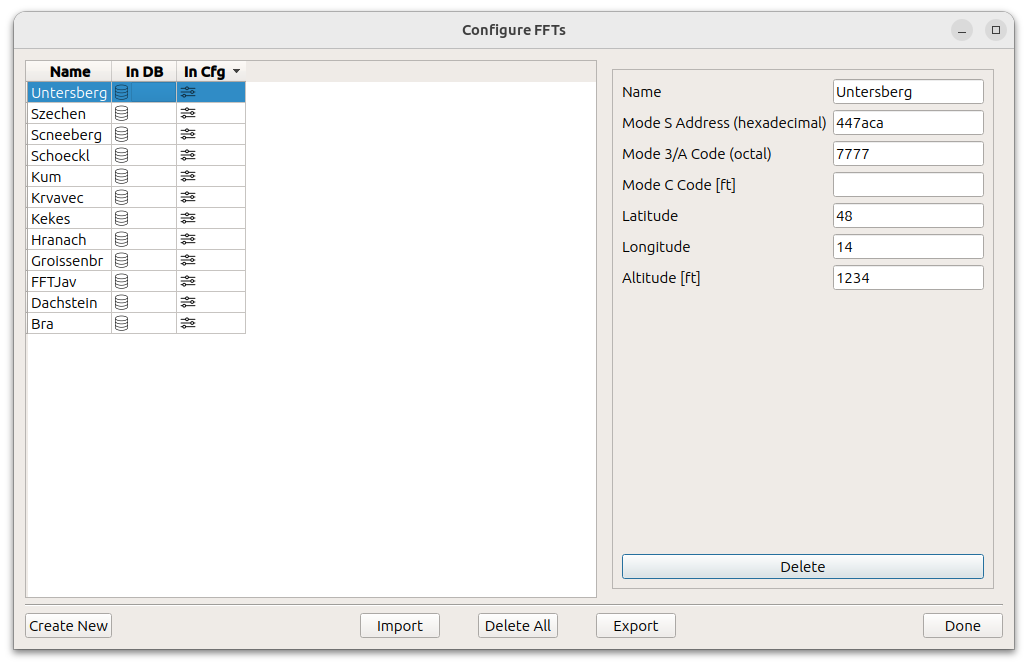
\includegraphics[width=18cm]{figures/configure_ffts.png}
  \caption{Configure Data Sources}
\end{figure}

The defined FFTs are used for:
\begin{itemize}
\item Display in OSGView
\item Usage of correct altitude information for Radar slant range correction during ASTERIX import
\end{itemize}
\ \\

All FFTs are always stored in the configuration as well as in the datebase, which means it is persistent and can be used in all new databases. It is useful to define all existing FFTs, since they are immediately used during import of data. \\

\paragraph {FFT Table Content}
\label{sec:configure_ffts_table_content}

\begin{itemize}
\item Name: Name of the data source
\item Mode S Address (hexadecimal): Optional
\item Mode 3/A Code (octal): Optional
\item Mode C Code [ft]: Optional
\item Latitude, Longitude: WGS84 position in degrees
\item Altitude [ft]: Altitude above MSL, in feet
\end{itemize}
\ \\

When a data source is selected in the table, additional details are shown in the right side, where edting is also possible. \\

Please \textbf{note} that all changes to a data sources are always written to the database as well as the configuration. \\

Depending on the DSType, additional information can be set in a source. For a non-Radar source, the following information is given:

\begin{itemize}
\item ID: Number indentifier (unique)
\item Network Line information
\begin{itemize}
    \item 4 different lines are possible, each with 
    \begin{itemize}
      \item Listen IP (defines used network interface and IGMP requests, optional when not using multicast)
      \item Multicast IP
      \item Multicast port
      \item Sender IP (optional, for filtering purposes)
    \end{itemize}
\end{itemize}
\end{itemize}
\ \\

Please note that for using real multicast addressess (inside of 224.0.0.0 to 239.255.255.255), it is recommended to also define the Listen IP to the local address of the network interface to be used. Otherwise the multicast data might not be received, or the wrong network interface might be used, causing COMPASS to receive no data. \\

Please note that if e.g. only Multicast IP and port are set, and the Multicast IP is set to a non-multicast one (outside of 224.0.0.0 to 239.255.255.255), a local replay is possible (without real multi-casting). \\

For sources of DSType 'Radar', the follwing additional information should be provided:

\begin{itemize}
\item Latitude: Source center position as WGS-84 latitude, as floating point number in degrees, e.g. 42.0001
\item Longitude: Source center position as WGS-84 longitude, as floating point number in degrees, e.g. 17.01
\item Altitude: Source center altitude above MSL, in meters
\end{itemize}
\ \\

Additional optional information can be provided:

\begin{figure}[H]
  \center
    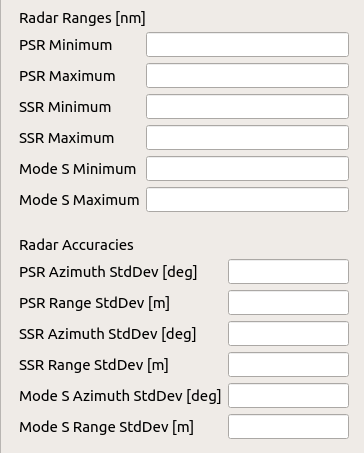
\includegraphics[width=8cm,frame]{figures/configure_data_sources_radar_details.png}
  \caption{Configure Data Sources: Radar details}
\end{figure}

\begin{itemize}
\item PSR Minimum: PSR minimum range, in nautical miles
\item PSR Maxmimum: PSR maximum range, in nautical miles
\item SSR Minimum: SSR minimum range, in nautical miles
\item SSR Maxmimum: SSR maximum range, in nautical miles
\item Mode S Minimum: Mode S minimum range, in nautical miles
\item Mode S Maxmimum: Mode S maximum range, in nautical miles
\item PSR Azimuth StdDev: PSR azimuth standard deviation, in degrees
\item PSR Range StdDev: PSR range standard deviation, in meters
\item SSR Azimuth StdDev: SSR azimuth standard deviation, in degrees
\item SSR Range StdDev: SSR range standard deviation, in meters
\item Mode S Azimuth StdDev: Mode S Radar azimuth standard deviation, in degrees
\item Mode S Range StdDev: Mode S Radar range standard deviation, in meters
\end{itemize}
\ \\

\subsubsection{Import/Export of Configuration Data Sources}
\label{sec:config_ds_export}

Using the 4 buttons on the bottom the following functions can be used:

\begin{itemize}
\item Export All: Export all configuration data sources as JSON file
\item Clear All: Delete all configuration data sources
\item Import: Import configuration data sources from JSON file
\item Auto Sync All to DB: Automatically synchronize all configuration data sources to database
\end{itemize}
\ \\

There are two versions of the data sources JSON file used for import/export. Please refer to \nameref{sec:appendix_data_sources}. \\

Using these functions, the configuration data sources can be changed for sensor context switches, or e.g. exported before an COMPASS version upgrade.
